
\chapter{Sampling-based Predictive Buffer Management}
\label{sec:PBM-sampling}

This chapter presents an alternative buffer management strategy based on sampling that uses the same estimates about future access times as PBM-PQ but removes the need for the approximate priority queue entirely. This improves prediction accuracy for choosing eviction candidates, significantly simplifies the design and implementation, and is more flexible and extensible.

\SetKw{KwReturn}{return}
\begin{algorithm}
\SetAlgoLined
\DontPrintSemicolon
\SetKwFunction{FEvictBlock}{ChooseEvictedBlock}
\SetKwFunction{FEstNextAccess}{EstimateNextAccess}
\SetKwFunction{FScanBlocksUntil}{scan\_blocks\_until}
\SetKwProg{Fn}{Function}{:}{}

\Fn{\FEvictBlock{}}{
    samples $\gets$ array of length $N$\;
    \For{$i \gets 1$ \KwTo $N$} {
       blk $\gets$ random unused block\;
       t $\gets$ \FEstNextAccess{blk}\;
       samples[$i$] $\gets$ (blk, t)\;
    }
    % sort(samples) descending by estimated access times\;
    \For{$i\gets 1$ \KwTo $N$}{
       $s \gets$ sample with highest estimated access time\;
       \eIf{$s$ can be evicted}{
          \KwReturn $s$\;
       }{
          remove $s$ from list of samples\;
       }
    }
    \KwReturn random unused block\;
}\;

\Fn{\FEstNextAccess{blk}}{
  \eIf{blk has registered scans}{
     \KwReturn      
     $\min_{s \in \text{blk.scans}}{\frac{s.\text{\FScanBlocksUntil{blk}}}{s.\text{est\_speed}}}$
     \;
  }{
     \KwReturn $\infty$\;
  }
}\;
\caption{Sampling-based eviction strategy}
\label{alg:sampling}
\end{algorithm}

The sampling-based approach, referred to in this thesis as PBM-sampling, tracks the progress of scans in the same way as PBM-PQ: scans are registered and a list of relevant scans is kept for each block. The change from PQ-based to sampling-based \gls{pbm} is in how it uses the estimated access times to select what to evict. Rather than use a data structure to rank candidates, the sampling-based strategy selects a random group of candidates and use the estimated access times to choose the victim from the selected sample.

Pseudocode for choosing which block to evict is shown in Algorithm~\ref{alg:sampling}. First, the system chooses $N$ random blocks from the cache that are not currently in use, where $N$ is a configurable constant.\footnote{$N=10$ for most experiments in the evaluation.} A block cannot be evicted if it is currently in use, so such blocks must be skipped and something else is selected. The sampling-based approach estimates the next access time for each of the $N$ blocks in the same way as PBM-PQ, by estimating when each active scan will reach the block and considering the scan that is predicted to reach it first. Then from the $N$ sampled blocks, the one with highest estimated next-access-time is returned.

Note that it is possible for the selected block to not be evictable anymore if a concurrent query either already evicted it or started using it. The implementation avoids locking the blocks when they are initially selected to minimize the possible impact on concurrent queries while calculating the access time estimates. To handle this race condition, there is a check at the end for whether the chosen block is still a valid candidate and another block is selected if it is not valid anymore.

This approach is similar in spirit to the learned relaxed Belady approach of \citet{relaxedBelady}. The next part of this chapter justifies why this approach is expected to work well.


\section{Generalizing the Optimal Eviction Strategy}
\label{sec:generalized-MIN}

The most straight-forward approach to mimic Belady's optimal caching policy MIN~\cite{beladyMIN} would be to try to identify the single cache item that will be accessed furthest in the future. However MIN only provides a single choice for eviction when there may be many optimal choices, making this approach more difficult to accomplish than it needs to be. To make the problem easier without sacrificing optimality, consider what MIN will eventually do with the items currently in the cache: any cache item that MIN would evict before that item is next accessed is also an optimal choice for eviction. This is established using the following lemmas:

% could move this to preamble...
\newtheorem{claim}{Lemma}

\begin{claim}\label{lemma:swap-opt}
% This can be generalized more: the policy does not have to be optimal, just that swapping two evictions in this situation will not change the hit rate. But here I only care about the optimal case.
Suppose that $A$ and $B$ are items in the cache at time-step $t_0$, both $A$ and $B$ are next accessed after $t_1$, and some optimal policy (not necessarily MIN) would evict $A$ at $t_0$ and evict $B$ at $t_1$. If the evictions of $A$ and $B$ are swapped -- so $B$ is evicted at $t_0$ and $A$ is evicted at $t_1$ instead -- then the resulting strategy is still optimal.
\end{claim}

\begin{proof}
Since neither $A$ nor $B$ are accessed between $t_0$ and $t_1$ and the rest of the cache contents are unaffected in this time range, swapping the evictions will not change the number of cache hits/misses between $t_0$ and $t_1$. After $t_1$ both $A$ and $B$ have been evicted and the cache contents are now identical to if the evictions were not swapped, so the behaviour after this point is identical to the original policy and there are also no additional cache misses after $t_1$. Thus $B$ would also be an optimal eviction candidate at $t_0$, since swapping these evictions does not occur any extra cache misses.
\end{proof}

Considering the above argument for MIN specifically instead of any optimal policy in general, then $A$ necessarily has a larger next access time at $t_0$ than $B$, since otherwise MIN would evict $B$ before $A$. This argument applies for \textit{all} items in the cache at $t_0$ that MIN would evict before their next access, so using Lemma \ref{lemma:swap-opt} they are \textit{all} optimal eviction choices at $t_0$. I refer to this set of cache items that MIN would evict before their next access as \textit{MIN-optimal}.


\begin{figure}
    \centering
    \includegraphics{figures/Diagrams/diagrams-belady-boundary.pdf}
    \caption[Higher next-access-time for MIN-optimal cache items]{Cache items evicted by MIN before next-access have later next-access time than items that will be read from the cache before eviction.}
    \label{fig:belady-boundary}
\end{figure}


\begin{claim}
\label{lemma:opt-greater-next-access}
% Using MIN, all cache items that would be evicted before their next access have later next-access-time than all other items in the cache.
All MIN-optimal cache items have later next-access-time than all items in the cache that are not MIN-optimal. (depicted in Figure \ref{fig:belady-boundary})
\end{claim}

\begin{proof}

Suppose $A$ and $B$ are items in the cache, and $B$ has earlier next-access-time than $A$. If $B$ is MIN-optimal, then $A$ must be as well.

Let $t^\text{evict}_A$ and $t^\text{evict}_B$ be the times when MIN would evict $A$ and $B$ respectively, and let $t^\text{access}_A$ and $t^\text{access}_B$ be the next access times of $A$ and $B$.

Suppose that $B$ is MIN-optimal so $t^\text{evict}_B < t^\text{access}_B$. As previously stated, $B$ is next accessed before $A$ so $t^\text{access}_B < t^\text{access}_A$, and as a result MIN will evict $A$ first so $t^\text{evict}_A < t^\text{evict}_B$. Then by transitivity, $t^\text{evict}_A < t^\text{access}_A$ so $A$ is also MIN-optimal.

Thus it is impossible for a MIN-optimal cache item to have earlier next-access-time than a non-MIN-optimal cache item.
\end{proof}

% [revise next para as it reads oddly: Then...  Then... ??]

Then at any time there are potentially many cache items that are optimal to evict, and some subset of optimal choices have next access times larger than all the other cache items. Based on this, there must be some cut-off time dividing these optimal-to-evict cache items from the rest -- depicted in Figure \ref{fig:belady-boundary} -- which if it were known would be very helpful in identifying good eviction candidates. This is similar to the ``Belady boundary'' described by \citet{relaxedBelady} as the minimum time-to-next-access of all items evicted by MIN. Unfortunately this cut-off time is not known in advance, but it is very useful to know that cache items with later next-access-time have a higher likelihood of being optimal eviction choices. 

Note also that even amongst items that MIN would not evict before their next access, it is still better to evict the one with larger access time. This is proven as part of the proof that MIN is optimal.~\cite{MINOptimality} % in Lemma 1 of the appendix

Thus, evicting the item with highest next-access-time from a sample makes sense and has a reasonably high chance of making an optimal decision assuming next-access-time estimates are accurate, and with a large enough sample. Suppose that the fraction of cache items that are optimal eviction candidates is $p$. Then the probability of making an optimal eviction choice is $1-(1-p)^N$ where $N$ is the sample size. Figure \ref{plot:P-opt-eviction} show the probability of optimal evictions as a function of $p$ for different sample sizes.

\begin{figure}
    \centering
    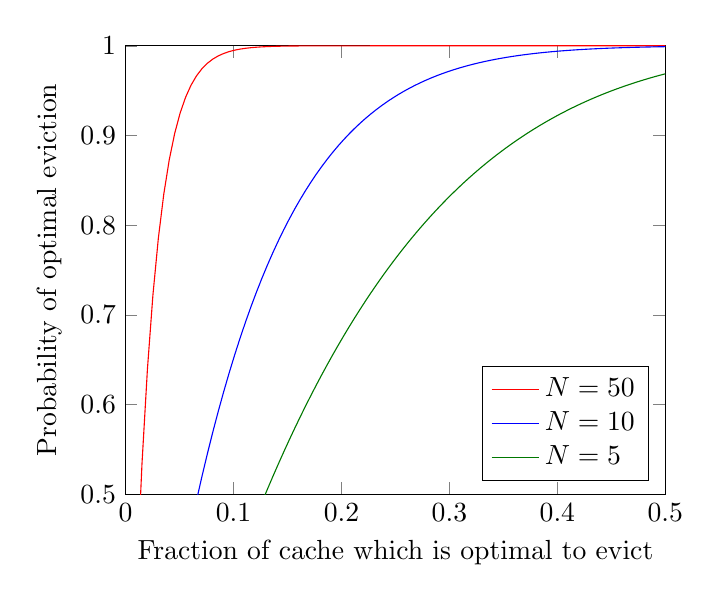
\begin{tikzpicture}
    \definecolor{darkgreen}{RGB}{0,120,0}
    \begin{axis}[
        domain=0:0.5, xmin=0, xmax=0.5,
        range=0.5:1, ymin=0.5, ymax=1,
        samples=100,
        legend pos=south east,
        legend cell align={left},
        xlabel=Fraction of cache which is optimal to evict,
        ylabel=Probability of optimal eviction,
    ]
    \addplot[color=red]{1-(1-x)^50};
    \addlegendentry{$N=50$};
    \addplot[color=blue]{1-(1-x)^10};
    \addlegendentry{$N=10$};
    \addplot[color=darkgreen]{1-(1-x)^5};
    \addlegendentry{$N=5$};
    \end{axis}
    \end{tikzpicture}
    \caption[PBM-sampling probability of optimal decision]{Probability of an optimal eviction decision with $N$ samples}
    \label{plot:P-opt-eviction}
\end{figure}



\subsection{Incompleteness of the generalized policy\label{subsec:gen-belady-incomplete}}

While the strategy of comparing next-access-time to when MIN would evict a cache item described in Chapter~\ref{sec:generalized-MIN} would identify more than one optimal eviction candidate, it is \textit{incomplete} in the sense that it does not identify \textit{all} possible optimal candidates, even with perfect knowledge of future accesses.

As an example of this: consider a cache of size 2 that initially contains items $A$ and $B$, and a sequence of accesses for item $C$, $A$, $B$, $A$. MIN would evict $B$ to read $C$, read $A$ from the cache, then evict $C$ to read $B$, and finally read $A$ from the cache again. This results in 2 evictions over the whole sequence. In the first step when $C$ is read, $A$ will be accessed before MIN would choose to evict it so only $B$ is MIN-optimal, not $A$.

However, it is possible to evict $A$ in the first step and still end up with an optimal sequence of evictions. Again starting with $A$ and $B$ in the cache, evict $A$ to read $C$, then evict $C$ to read $A$, and for the last two reads $B$ and $A$ are cached. This sequence of accesses also has only 2 evictions, so it is optimal, but it does not evict only MIN-optimal candidates. Thus the generalized policy is \textit{incomplete} in that it does not identify all possible optimal eviction decisions.

\subsection{Eviction times of the generalized policy}
An interesting observation is that the generalized policy will have its cache misses and evictions at the same time steps in the access sequence as MIN. However, for the example in Chapter~\ref{subsec:gen-belady-incomplete} of an optimal sequence of evictions that does not follow the generalized optimal policy, the evictions occur earlier in the sequence, at the first and second access instead of first and third. 

% This raises a few follow up questions that I do not explore in this thesis:
% \begin{enumerate}
%     \item Does MIN always have the latest possible evictions?
%     \item Is there sequence of evictions that does not follow the generalized optimal policy, but is still optimal and does not evict earlier than MIN?
%     \item Knowing the future accesses, is it possible to efficiently identify \textit{all} optimal eviction choices at a particular time?
% \end{enumerate}


\section{Sampling-based PBM: Benefits and Trade-offs\label{sec:sampling-advantages}}

To maximize performance, the buffer management policy should maximize the hit rate of block accesses while minimizing CPU overhead. This includes minimizing the time to choose what to evict, time to maintain metadata, and limit time holding locks so that threads can allocate cache blocks concurrently without waiting for each other.

PBM-PQ~\cite{pbm} trades off prediction accuracy by using the approximate priority queue to avoid the high CPU overhead of maintaining an exact priority queue, and allowing estimates to become stale. Sampling-based \gls{pbm} benefits from removing the central priority-queue data structure, allowing it to achieve better hit rate without additional CPU overhead.


\textbf{Simplicity}: The most obvious advantage after implementing both policies is increased simplicity -- sampling removes the entire approximate priority queue data structure along with the maintenance required to shift the buckets periodically and ensure block groups are in the correct bucket as blocks move in and out of the cache or their registered scan set changes.

With sampling, all of this is removed and the eviction logic changes, with almost nothing added. In the PostgreSQL implementations, PBM-sampling has about 600 fewer lines of code than PBM-PQ.


\textbf{Freshness of access-time estimates}: The sampling-based approach computes next-access-time estimates as late as possible -- only when a block is being considered for immediate eviction -- so the estimates it uses are based on the most up-to-date information available.

In contrast, the PQ-based approach calculates estimates only when the set of scans registered for a block changes potentially causing the block to be moved to a different bucket of the approximate priority queue. If the initial estimated access times were perfectly accurate this would not matter, but in practice the scans will change speed over time depending on various run-time factors. A block could remain in the cache for minutes at a time without its position in the queue being recalculated, leaving plenty of time for estimates to drift. Less accurate estimates lead to worse eviction decisions and, by extension, worse performance.

\textbf{Accuracy of access-time estimates}: The approximate priority queue considers blocks in the same bucket as equivalent when deciding what to evict, with buckets further in the future -- which are checked first for potential eviction candidates -- representing exponentially larger time ranges. Sampling compares the exact estimated next-access, however, it considers only a small sample of blocks for each eviction compared to PBM-PQ, which chooses among all blocks in the cache. Both methods sacrifices some precision that prevents them from always picking the best block to evict, even if the estimates were completely accurate. Chapter~\ref{sec:generalized-MIN} discusses how to reason about the precision of the sampling-based strategy.  % less clear how to reason about it for PQ-based

\textbf{Extensibility}: PBM-PQ is designed for workloads with mostly sequential scans, and the approximate priority queue makes it difficult to extend it to other workloads. \citet{pbm} suggest, but do not implement, a way to incorporate frequency statistics to handle blocks that are not requested by sequential scans but may be accessed by other methods for hybrid workloads. Their proposal requires an entire new data structure that is processed differently from the existing priority queue because the existing structure assumes the priorities (time to next access) change in a specific way over time. 

With sampling, a complex data structure is not required for ordering blocks, so it is much easier to extend to support other workload types. Unlike with PBM-PQ, no extra work is required to make use of improved assess time estimates using new sources of information.

\textbf{Tunability}: With sampling, the sample size can be changed at run-time without interrupting the workload in any way. Caching policies must compromise between CPU cost and hit rate, and adjusting the sample size is an easy way to do this with intuitive impact: more samples should increase the hit rate, but increases the per-eviction CPU cost.

With PBM-PQ, the number of buckets in the queue and the time ranges represented by each bucket are adjustable. However, changing these parameters requires modifying the data structure including potentially recalculating access time estimates, and it is not as obvious when more buckets or a different time range would be beneficial. These adjustments improve the precision, but do not help when estimates become stale.


\textbf{Concurrency:} PBM-sampling does not have a central data structure used for making eviction decisions, so evictions can be done in parallel from multiple processes with low frequency of one thread having to wait for another (one thread will have to wait if two threads randomly sample the same buffer at the same time). Using the approximate priority queue prevents concurrent evictions, which could potentially limit the scalability at high levels of concurrency. PBM-PQ works around this limitation by evicting many blocks at once so that allocating a buffer usually does not need to wait.% and in the experiments the centralized data structure of the PQ-based implementation does not seem to actually impact performance.

 % ... cpu overhead more generally? ... Measured average CPU overhead of choosing eviction candidate lower for sampling, but not as low as clock. -- calculates priorities more frequently ...


% \textbf{Disadvantages}: ... are there any? (other than weird issues where it does not help on HDD...)
